\chapter{Entwicklung der Schl�sselelemente}
\section{�bersicht des gesamten Modells}

\section{Schaltplan}

\section{BMS und Laden}

\section{Mecanum}

\section{Planetengetriebe}

\section{ESP-32 vs. ESP-8266}

\section{User-Interface}
\subsection{Java (obsolet)}

\subsection{HTML5 und Controller-Anbindung}

Das Java Programm wurde aus mehreren Gr�nden zugunsten einer auf HTML5, sowie JavaScript basierten Weboberfl�che ersetzt:\par

\begin{itemize}
	\item Native und einheitliche Unterst�tzung f�r Controller unterschiedlichster Marken in HTML5\par
	
	\item Unabh�ngig von Java Laufzeitumgebung, sowie Verf�gbarkeit des Programms.\\
	(Hierbei muss nur ein Browser auf dem PC installiert sein.)\par
	
	\item Einfache �bertragung der Daten per WebSockets anstatt von "raw"  Sockets, ohne ein eigenes "Frame"  um die Daten bauen zu m�ssen
\end{itemize}\par


\vspace{\baselineskip}
Dies l�sst sich sehr leicht durch die ESPAsyncWebServer Library f�r den ESP32 l�sen. \par

Diese hostet direkt auf dem ESP32 einen WebServer der sowohl HTML5, JS, als auch CSS bereitstellen kann. Als Speicherort f�r diese Dateien wird das sogenannte Dateisystem SPIFFS verwendet, welches den Flashspeicher des ESP32 als Dateisystem benutzt, wie es beispielsweise aus Windows bekannt ist.\par

Eine Einschr�nkung ist die Limitierung auf eine gleichzeitige Verbindung zu dem Server. Dies wurde empirisch herausgefunden und somit konnte nicht sicher gesagt werden, ob es sich hier um eine Einschr�nkung aufgrund von mangelnder Rechenleistung handelt oder ob die Library nicht mehr unterst�tzt. Als L�sung dieses Problems, ist nun die Anzahl der Verbindungen die der WiFi Accesspoint akzeptiert, auf eins gesetzt.\par


\vspace{\baselineskip}

\begin{figure}[!ht]
	\centering
	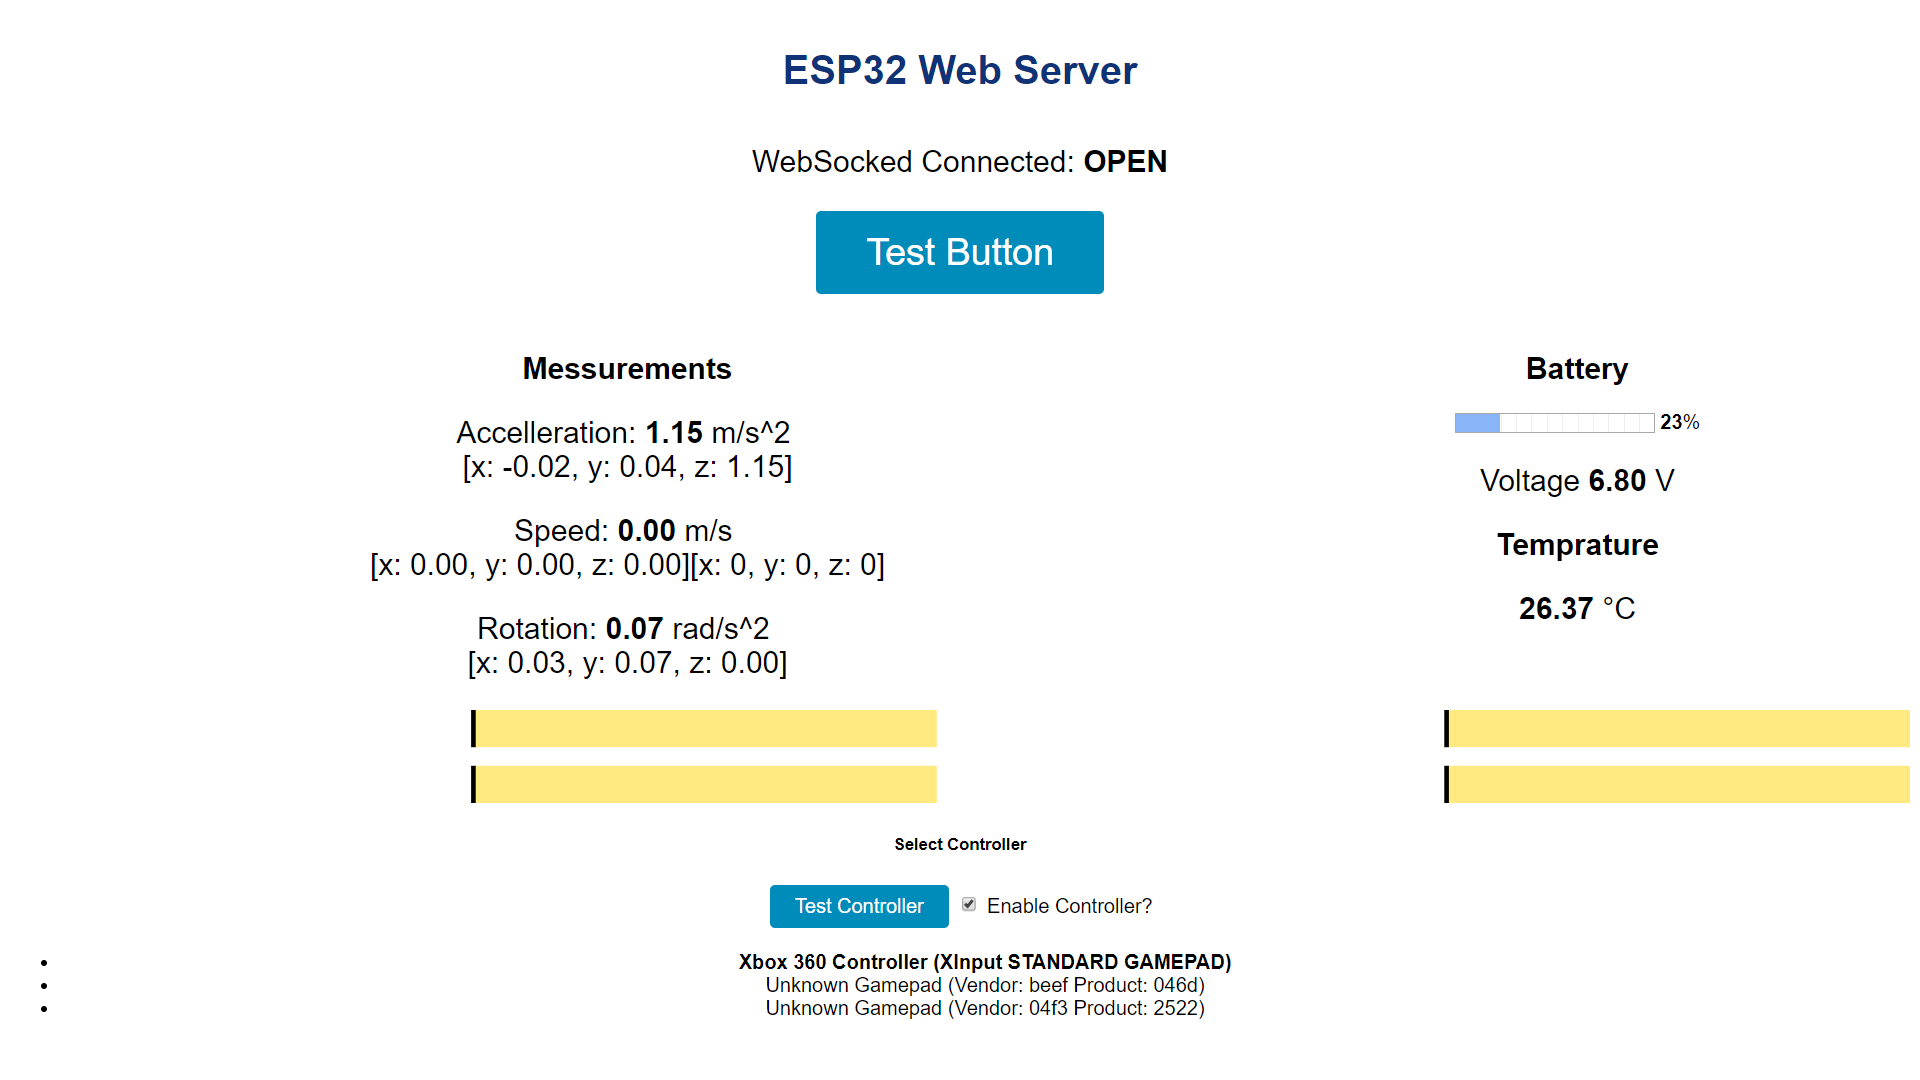
\includegraphics[width=\textwidth]{bilder/WebValues.png}
	\caption{Bildschirmfoto Weboberfl�che}
	\label{bild:webvalues}
\end{figure}

In der Weboberfl�che (siehe Abbildung \ref{bild:webvalues}) sind ebenfalls noch jegliche Messwerte hinterlegt, die das Fahrzeug sammelt.\par

Diese sind:\par

\begin{itemize}
	\item Beschleunigung 
	\item Geschwindigkeit
	\item Rotationsgeschwindigkeit
	\item Batteriespannung
	\item Temperatur
	\item Drehgeschwindigkeit der jeweiligen Motoren
\end{itemize}\par


\vspace{\baselineskip}
F�r die Wahl des Controllers ist eine ausw�hlbare Liste aller angeschlossenen Controller am Ende der Seite vorhanden. Falls der Nutzer keinen Controller besitzt oder angeschlossen hat, kann durch das Abw�hlen der Checkbox auf die Steuerung per WASD, sowie die Pfeiltasten gewechselt werden.\par

\subsection{Protokoll}
Zum �bertragen wurde ein bin�res Protokoll ausgew�hlt, um die Datenrate gering zu halten, sowie die Verarbeitung auf dem Microcontroller zu vereinfachen.\par

Da durch Websockets bereits ein Integrierter Frame geschickt wird, muss nicht bei jeder Nachricht die L�nge und Anfangs- und Endbyte mitgeschickt werden, wie es sonst bei raw Sockets n�tig gewesen w�re.\par

Hierbei wird jeder Wert als Int16 geschickt, um ein ausreichend gro�es Spektrum bei geringer Datenrate zu gew�hrleisten. \par

Am Anfang jeder Nachricht wird die ID ebenfalls als int16 geschickt, somit w�ren 65536 unterschiedliche Nachrichten erlaubt.\par

Um die Anzahl an Nachrichten zu verringern, wurden die Batteriespannung und Werte des Gyroskop zu einer kombinierte Nachricht zusammengefasst, um den Overhead gering zu halten.\par

\begin{table}[ht]
	\centering
	\resizebox{\textwidth}{!}{
\begin{tabular}{|c|c|c|c|c|c|c|c|c|c|c|c|c|}
	\hline 
	Name & ID & \multicolumn{11}{c|}{Werte} \\ 
	\hline 
	\hline 
	DRIVE & 0 & X-Achse L & Y-Achse L & X-Achse R & Y-Achse R &  &  &  &  &  &  &  \\ 
	\hline 
	GYRO & 1 & Speed - X & Speed - Y & Speed - Z & Accel - X & Accel - Y & Accel - Z & Rot - X & Rot - Y & Rot - Z  &  & \\ 
	\hline 
	BATTERY & 2 & Voltage &  &  &  &  &  &  &  &  &  &  \\ 
	\hline 
	MOTOR & 3 & Speed - M1 & Speed - M2 & Speed - M3 & Speed - M4 &  &  &  &  &  &  &  \\ 
	\hline 
	COMB & 4 & Speed - X & Speed - Y & Speed - Z & Accel - X & Accel - Y & Accel - Z & Rot - X & Rot - Y & Rot - Z  & Battery & Temp \\ 
	\hline 
\end{tabular}} 
\caption{Bin�res Protokoll} 
\end{table} 



\section{Steuerung per (XBox) Controller}

\section{PLA vs. TPU}

\section{Eierhalter}					

\section{Leichtbau}	